Nick Vosseteig

2014-10-31

building, wiring, programming

\begin{tabular}{|p{5cm}|p{5cm}|}
 \hline
 building&
I continued building the robot and added the spinning prototype on the front.
 \\
 \hline
wiring&
I wired the motor for the spinning intake device.
 \\
 \hline
programming&
I added to the robot's code to make the 1 and 2 buttons on the controller control the intake device.
 \\
 \hline
\end{tabular}

\section*{Programming}
I added this section of code to get the spinner to work:
\begin{lstlisting}[style = RobotC]	
	if(joy1Btn(2)){
		motor[intake] = 100;
		}else if(joy1Btn(1)){
		motor[intake] = -100;
		}else{
		motor[intake] = 0;
	}
\end{lstlisting}
This week we tested out the code and got all the  motors working. There was one bad motor which we replaced, and then the motors were not assigned correctly in the code. We just went through and tested each one individually to correct it.

\section*{Building and wiring}
This week we mainly built more on the robot frame and added the prototype intake device on the front:

\begin{center}
 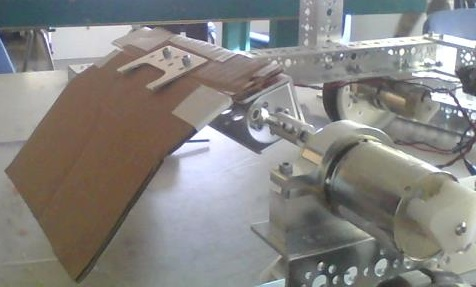
\includegraphics[width=215px]{./Entries/Images/intake_device2.jpg}
\end{center}